\documentclass[12pt,oneside]{book}

\usepackage{../../lib/tex/naproche}
\usepackage{../../lib/tex/libraries}
\usepackage{../../lib/tex/basic-notions}
\usepackage{graphicx}
\usepackage{float}
\usepackage{caption}


\title{Set theory}
\author{Marcel Schütz}
\date{2022}

\begin{document}
  \maketitle

  \tableofcontents

  \paragraph*{}
  \begin{figure}[H]
    \centering
    \fbox{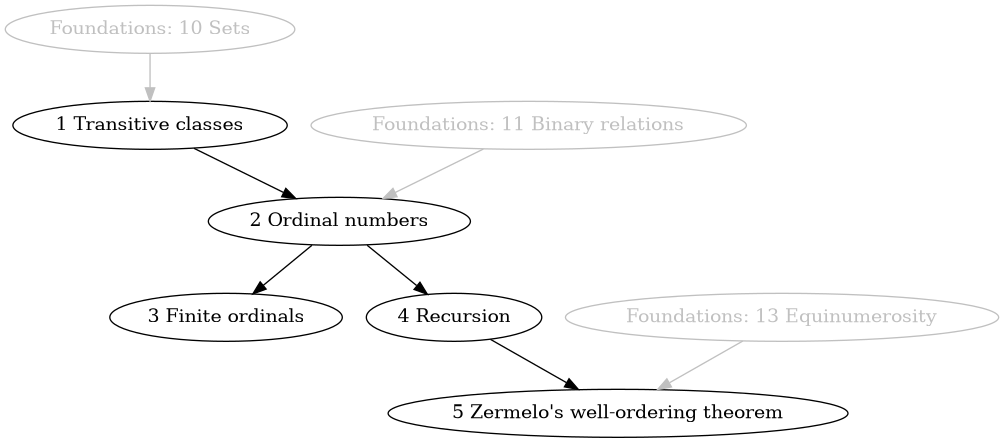
\includegraphics[width=0.9\textwidth]{./dependency-graph/graph.png}}
    \caption*{Interdependencies of the chapters}
  \end{figure}

  \subfile{sections/01_transitive-classes.ftl.tex}
  \subfile{sections/02_ordinals.ftl.tex}
  \subfile{sections/03_finite-ordinals.ftl.tex}
\end{document}
